\documentclass{standalone}
\usepackage{tikz}
\usetikzlibrary{patterns, positioning}
\usepackage[sfdefault]{ClearSans} %% option 'sfdefault' activates Clear Sans as the default text font
\usepackage[T1]{fontenc}

\begin{document}
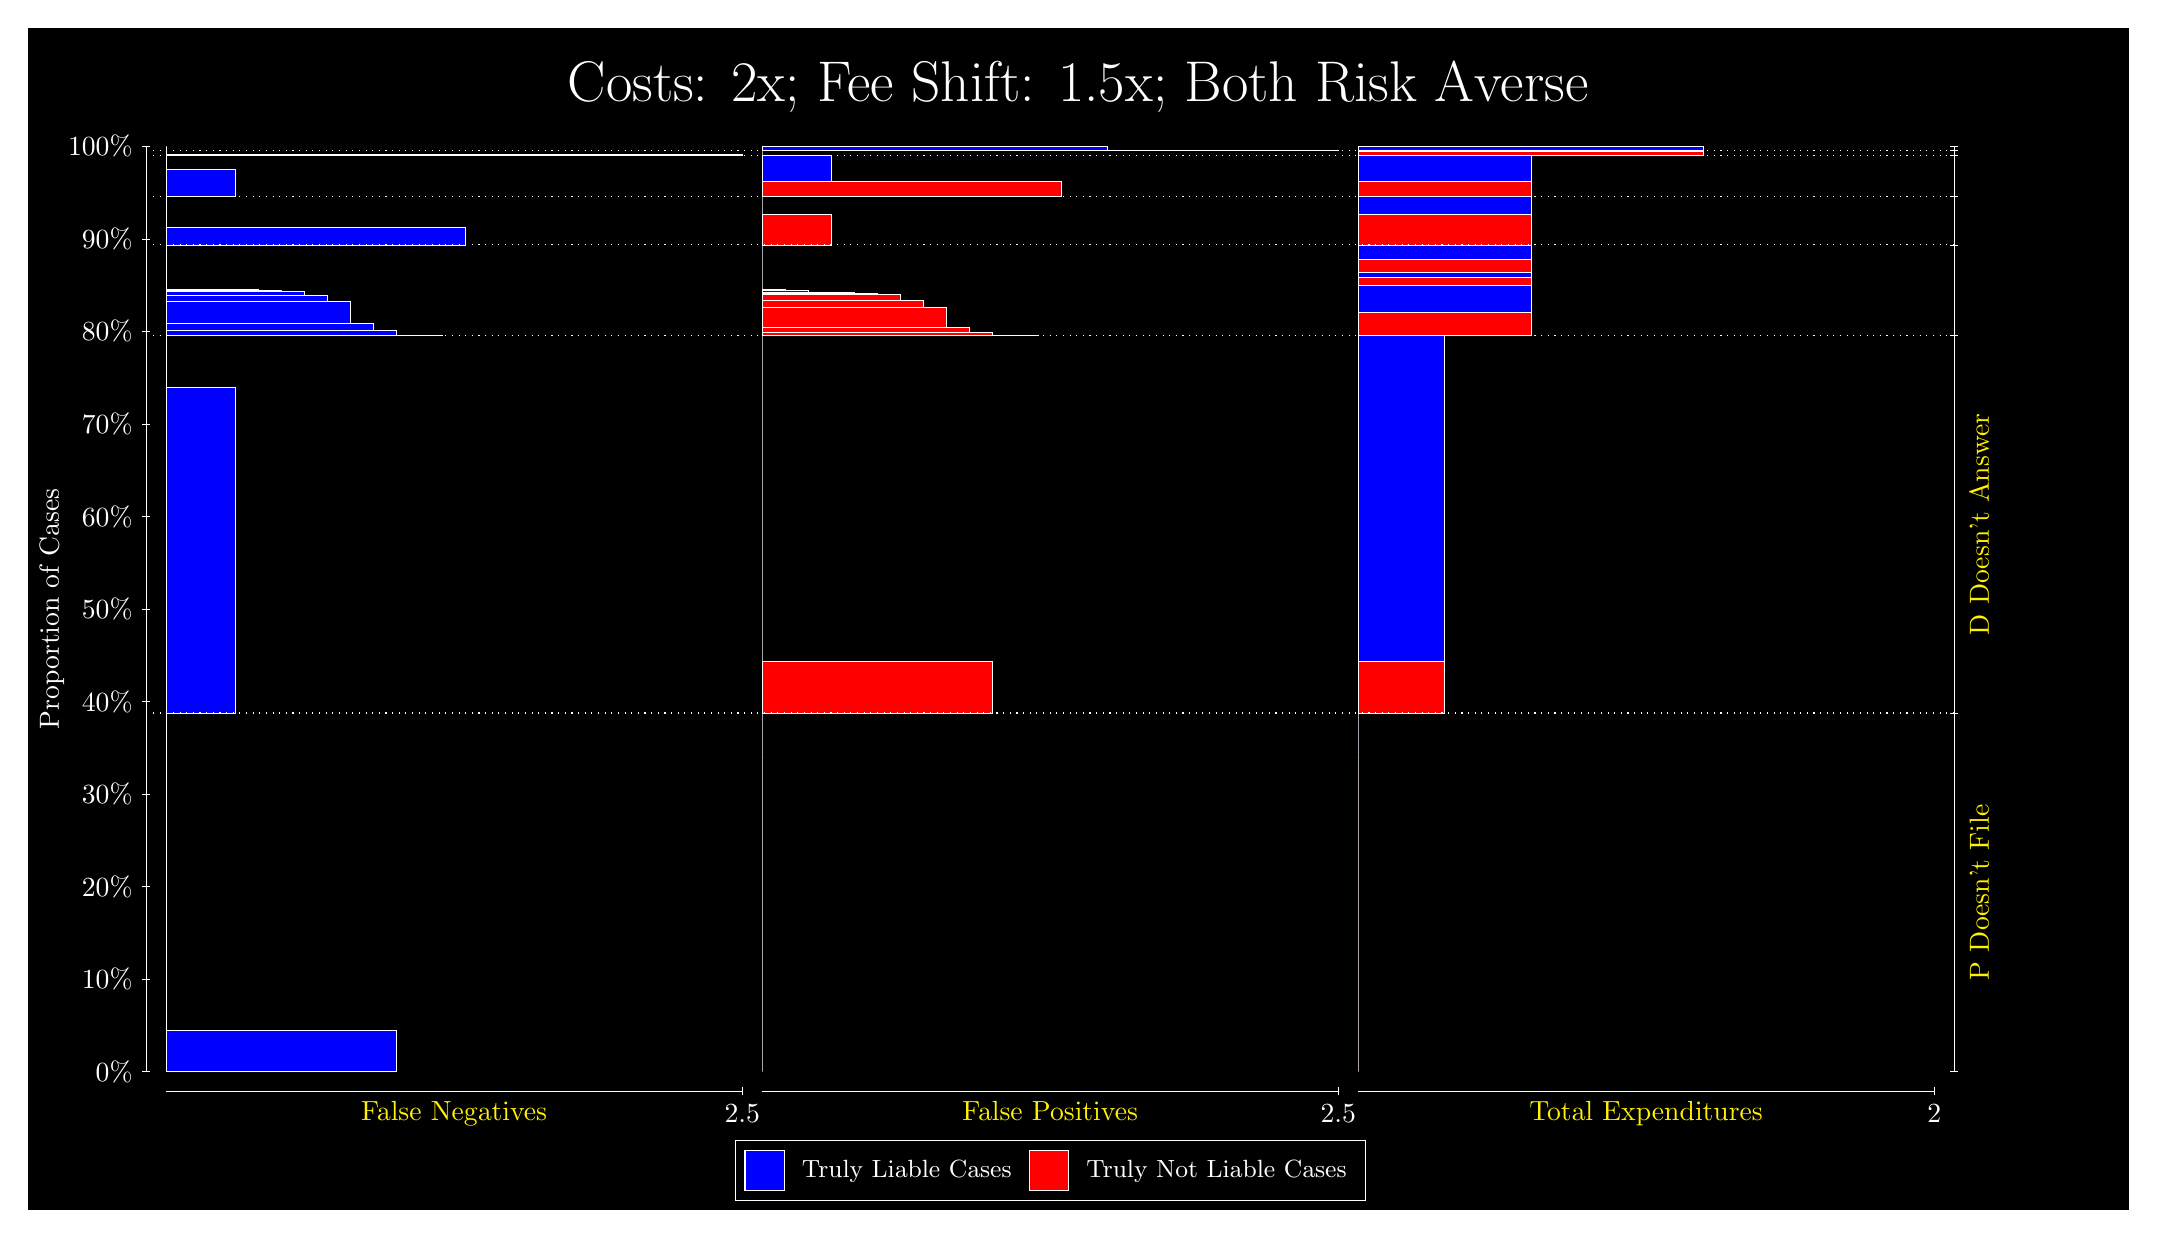
\begin{tikzpicture}
\draw[fill=black] (0,0) rectangle (26.667,15);
\draw[text=white] (0,13.5) rectangle (26.667,15) node[midway] {\huge Costs: 2x; Fee Shift: 1.5x; Both Risk Averse};
\draw[white, very thin] (1.5,1.75) -- (1.5,13.5);
\node[rotate=90, text=white, anchor=center] at (0.3, 7.625) {Proportion of Cases};
\draw[white, very thin] (1.45,1.75) -- (1.55,1.75);
\node[text=white, anchor=east] at (1.45, 1.75) {0\%};
\draw[white, very thin] (1.45,2.925) -- (1.55,2.925);
\node[text=white, anchor=east] at (1.45, 2.925) {10\%};
\draw[white, very thin] (1.45,4.1) -- (1.55,4.1);
\node[text=white, anchor=east] at (1.45, 4.1) {20\%};
\draw[white, very thin] (1.45,5.275) -- (1.55,5.275);
\node[text=white, anchor=east] at (1.45, 5.275) {30\%};
\draw[white, very thin] (1.45,6.45) -- (1.55,6.45);
\node[text=white, anchor=east] at (1.45, 6.45) {40\%};
\draw[white, very thin] (1.45,7.625) -- (1.55,7.625);
\node[text=white, anchor=east] at (1.45, 7.625) {50\%};
\draw[white, very thin] (1.45,8.8) -- (1.55,8.8);
\node[text=white, anchor=east] at (1.45, 8.8) {60\%};
\draw[white, very thin] (1.45,9.975) -- (1.55,9.975);
\node[text=white, anchor=east] at (1.45, 9.975) {70\%};
\draw[white, very thin] (1.45,11.15) -- (1.55,11.15);
\node[text=white, anchor=east] at (1.45, 11.15) {80\%};
\draw[white, very thin] (1.45,12.325) -- (1.55,12.325);
\node[text=white, anchor=east] at (1.45, 12.325) {90\%};
\draw[white, very thin] (1.45,13.5) -- (1.55,13.5);
\node[text=white, anchor=east] at (1.45, 13.5) {100\%};

\draw[white, very thin] (24.457,1.75) -- (24.457,13.5);
\draw[white, very thin] (24.407,1.75) -- (24.507,1.75);
\node[anchor=west] at (24.407, 1.75) {};
\draw[white, very thin] (24.407,6.3037) -- (24.507,6.3037);
\node[anchor=west] at (24.407, 6.3037) {};
\draw[white, very thin] (24.407,11.094) -- (24.507,11.094);
\node[anchor=west] at (24.407, 11.094) {};
\draw[white, very thin] (24.407,12.248) -- (24.507,12.248);
\node[anchor=west] at (24.407, 12.248) {};
\draw[white, very thin] (24.407,12.866) -- (24.507,12.866);
\node[anchor=west] at (24.407, 12.866) {};
\draw[white, very thin] (24.407,13.387) -- (24.507,13.387);
\node[anchor=west] at (24.407, 13.387) {};
\draw[white, very thin] (24.407,13.445) -- (24.507,13.445);
\node[anchor=west] at (24.407, 13.445) {};
\draw[white, very thin] (24.407,13.5) -- (24.507,13.5);
\node[anchor=west] at (24.407, 13.5) {};

\draw[white, very thin, fill=blue] (1.75,1.75) rectangle (4.6775,2.2783);
\draw[white, very thin, fill=red] (1.75,2.2783) rectangle (1.75,6.3037);
\draw[white, very thin, fill=blue] (1.75,6.3037) rectangle (2.6283,10.434);
\draw[white, very thin, fill=red] (1.75,10.434) rectangle (1.75,11.094);
\draw[white, very thin, fill=blue] (1.75,11.094) rectangle (5.2631,11.099);
\draw[white, very thin, fill=blue] (1.75,11.099) rectangle (4.9703,11.104);
\draw[white, very thin, fill=blue] (1.75,11.104) rectangle (4.6775,11.161);
\draw[white, very thin, fill=blue] (1.75,11.161) rectangle (4.3848,11.164);
\draw[white, very thin, fill=blue] (1.75,11.164) rectangle (4.3848,11.254);
\draw[white, very thin, fill=blue] (1.75,11.254) rectangle (4.092,11.533);
\draw[white, very thin, fill=blue] (1.75,11.533) rectangle (3.7993,11.608);
\draw[white, very thin, fill=blue] (1.75,11.608) rectangle (3.5065,11.658);
\draw[white, very thin, fill=blue] (1.75,11.658) rectangle (3.2138,11.669);
\draw[white, very thin, fill=blue] (1.75,11.669) rectangle (2.921,11.69);
\draw[white, very thin, fill=red] (1.75,11.69) rectangle (1.75,12.248);
\draw[white, very thin, fill=blue] (1.75,12.248) rectangle (5.5558,12.476);
\draw[white, very thin, fill=red] (1.75,12.476) rectangle (1.75,12.866);
\draw[white, very thin, fill=blue] (1.75,12.866) rectangle (2.6283,13.203);
\draw[white, very thin, fill=red] (1.75,13.203) rectangle (1.75,13.387);
\draw[white, very thin, fill=blue] (1.75,13.387) rectangle (9.0689,13.398);
\draw[white, very thin, fill=red] (1.75,13.398) rectangle (1.75,13.445);
\draw[white, very thin, fill=red] (1.75,13.445) rectangle (1.75,13.455);
\draw[white, very thin, fill=blue] (1.75,13.455) rectangle (1.75,13.5);
\draw[white, very thin, fill=red] (9.3189,1.75) rectangle (9.3189,5.7754);
\draw[white, very thin, fill=blue] (9.3189,5.7754) rectangle (9.3189,6.3037);
\draw[white, very thin, fill=red] (9.3189,6.3037) rectangle (12.246,6.9639);
\draw[white, very thin, fill=blue] (9.3189,6.9639) rectangle (9.3189,11.094);
\draw[white, very thin, fill=red] (9.3189,11.094) rectangle (12.832,11.098);
\draw[white, very thin, fill=red] (9.3189,11.098) rectangle (12.539,11.105);
\draw[white, very thin, fill=red] (9.3189,11.105) rectangle (12.246,11.142);
\draw[white, very thin, fill=red] (9.3189,11.142) rectangle (11.954,11.208);
\draw[white, very thin, fill=red] (9.3189,11.208) rectangle (11.661,11.461);
\draw[white, very thin, fill=red] (9.3189,11.461) rectangle (11.368,11.551);
\draw[white, very thin, fill=red] (9.3189,11.551) rectangle (11.075,11.619);
\draw[white, very thin, fill=red] (9.3189,11.619) rectangle (10.783,11.629);
\draw[white, very thin, fill=red] (9.3189,11.629) rectangle (10.49,11.652);
\draw[white, very thin, fill=blue] (9.3189,11.652) rectangle (9.9044,11.673);
\draw[white, very thin, fill=blue] (9.3189,11.673) rectangle (9.6116,11.684);
\draw[white, very thin, fill=blue] (9.3189,11.684) rectangle (9.3189,12.248);
\draw[white, very thin, fill=red] (9.3189,12.248) rectangle (10.197,12.638);
\draw[white, very thin, fill=blue] (9.3189,12.638) rectangle (9.3189,12.866);
\draw[white, very thin, fill=red] (9.3189,12.866) rectangle (13.125,13.051);
\draw[white, very thin, fill=blue] (9.3189,13.051) rectangle (10.197,13.387);
\draw[white, very thin, fill=red] (9.3189,13.387) rectangle (9.3189,13.434);
\draw[white, very thin, fill=blue] (9.3189,13.434) rectangle (9.3189,13.445);
\draw[white, very thin, fill=red] (9.3189,13.445) rectangle (16.638,13.455);
\draw[white, very thin, fill=blue] (9.3189,13.455) rectangle (13.71,13.5);
\draw[white, very thin, fill=red] (16.888,1.75) rectangle (16.888,5.7754);
\draw[white, very thin, fill=blue] (16.888,5.7754) rectangle (16.888,6.3037);
\draw[white, very thin, fill=red] (16.888,6.3037) rectangle (17.986,6.9639);
\draw[white, very thin, fill=blue] (16.888,6.9639) rectangle (17.986,11.094);
\draw[white, very thin, fill=red] (16.888,11.094) rectangle (19.083,11.392);
\draw[white, very thin, fill=blue] (16.888,11.392) rectangle (19.083,11.731);
\draw[white, very thin, fill=red] (16.888,11.731) rectangle (19.083,11.835);
\draw[white, very thin, fill=blue] (16.888,11.835) rectangle (19.083,11.904);
\draw[white, very thin, fill=red] (16.888,11.904) rectangle (19.083,12.061);
\draw[white, very thin, fill=blue] (16.888,12.061) rectangle (19.083,12.248);
\draw[white, very thin, fill=red] (16.888,12.248) rectangle (19.083,12.638);
\draw[white, very thin, fill=blue] (16.888,12.638) rectangle (19.083,12.866);
\draw[white, very thin, fill=red] (16.888,12.866) rectangle (19.083,13.051);
\draw[white, very thin, fill=blue] (16.888,13.051) rectangle (19.083,13.387);
\draw[white, very thin, fill=red] (16.888,13.387) rectangle (21.279,13.434);
\draw[white, very thin, fill=blue] (16.888,13.434) rectangle (21.279,13.445);
\draw[white, very thin, fill=red] (16.888,13.445) rectangle (21.279,13.455);
\draw[white, very thin, fill=blue] (16.888,13.455) rectangle (21.279,13.5);
\draw[white, dotted] (1.5,6.3037) -- (24.457,6.3037);
\draw[white, dotted] (1.5,11.094) -- (24.457,11.094);
\draw[white, dotted] (1.5,12.248) -- (24.457,12.248);
\draw[white, dotted] (1.5,12.866) -- (24.457,12.866);
\draw[white, dotted] (1.5,13.387) -- (24.457,13.387);
\draw[white, dotted] (1.5,13.445) -- (24.457,13.445);
\draw[white, very thin] (1.75,1.5) -- (9.0689,1.5);
\node[text=yellow, anchor=north] at (5.4094, 1.5) {False Negatives};
\draw[white, very thin] (9.0689,1.45) -- (9.0689,1.55);
\node[text=white, anchor=north] at (9.0689, 1.45) {2.5};

\draw[white, very thin] (9.3189,1.5) -- (16.638,1.5);
\node[text=yellow, anchor=north] at (12.978, 1.5) {False Positives};
\draw[white, very thin] (16.638,1.45) -- (16.638,1.55);
\node[text=white, anchor=north] at (16.638, 1.45) {2.5};

\draw[white, very thin] (16.888,1.5) -- (24.207,1.5);
\node[text=yellow, anchor=north] at (20.547, 1.5) {Total Expenditures};
\draw[white, very thin] (24.207,1.45) -- (24.207,1.55);
\node[text=white, anchor=north] at (24.207, 1.45) {2};

\node[text=yellow, centered, rotate=90] at (24.777, 4.0269) {P Doesn't File};
\node[text=yellow, centered, rotate=90] at (24.777, 8.6989) {D Doesn't Answer};






\draw (12.978300999999998,1.5) node[draw=none] (baseCoordinate) {};
\begin{scope}[align=center]
        \matrix[scale=0.5, draw=white, below=0.5cm of baseCoordinate, nodes={draw}, column sep=0.1cm]{
            \node[rectangle, draw, minimum width=0.5cm, minimum height=0.5cm, fill=blue] {}; &
            \node[draw=none, font=\small, text=white] (B) {Truly Liable Cases}; &
            \node[rectangle, draw, minimum width=0.5cm, minimum height=0.5cm, fill=red] {}; &
            \node[draw=none, font=\small, text=white] (B) {Truly Not Liable Cases}; \\
            };
\end{scope}

\end{tikzpicture}
\end{document}